\def\year{2015}
%File: formatting-instruction.tex
\documentclass[letterpaper]{article}
\usepackage{aaai}
\usepackage{times}
\usepackage{helvet}
\usepackage{courier}
\usepackage{graphicx}
\frenchspacing
\setlength{\pdfpagewidth}{8.5in}
\setlength{\pdfpageheight}{11in}
\pdfinfo{
/Title (Insert Your Title Here)
/Author (Put All Your Authors Here, Separated by Commas)}
\setcounter{secnumdepth}{0}  
 \begin{document}
% The file aaai.sty is the style file for AAAI Press 
% proceedings, working notes, and technical reports.
%
\title{Formatting Instructions \\for Authors Using \LaTeX{}}
\author{AAAI Press\\
Association for the Advancement of Artificial Intelligence\\
2275 East Bayshore Road, Suite 160\\
Palo Alto, California 94303\\
}
\maketitle
\begin{abstract}
\begin{quote}
AAAI creates proceedings, working notes, and technical reports directly from electronic source furnished by the authors. To ensure that all papers in the publication have a uniform appearance, authors must adhere to the following instructions. 
\end{quote}
\end{abstract}

\noindent Congratulations on having a paper selected for inclusion in an AAAI Press proceedings or technical report! This document details the requirements necessary to get your accepted paper published using \LaTeX{}. If you are using Microsoft Word, instructions are provided in a different document. If you want to use some other formatting software, you must obtain permission from AAAI Press first. 

The instructions herein are provided as a general guide for experienced \LaTeX{} users who would like to use that software to format their paper for an AAAI Press publication or report. If you are not an experienced \LaTeX{} user, do not use it to format your paper. AAAI cannot provide you with support and the accompanying style files are \textbf{not} guaranteed to work. If the results you obtain are not in accordance with the specifications you received, you must correct your source file to achieve the correct result. 

These instructions are generic. Consequently, they do not include specific dates, page charges, and so forth. Please consult your specific written conference instructions for details regarding your submission. Please review the entire document for specific instructions that might apply to your particular situation. All authors must comply with the following:

\begin{itemize}
\item You must use the latest AAAI Press \LaTeX{} macro.
\item Download the author kit.
\item Complete, sign, and return by the deadline the AAAI copyright form (proceedings authors) or distribution license (technical report authors).
\item Read and format your paper source and PDF according to the formatting instructions for authors.
\item Submit your electronic files and abstract using our electronic submission form \textbf{on time.}
\item Submit your copyright form, and any required page or formatting charges to AAAI Press so that they are received by the deadline.
\item Check every page of your paper before submitting it.
\end{itemize}

\section{Copyright}
All papers submitted for publication by AAAI Press must be accompanied by a valid signed copyright form or, in the case of technical reports, by a valid signed permission to distribute form. There are no exceptions to this requirement. You must send us the original version of this form. However, to meet the deadline, you may fax (1-650-321-4457) or scan and e-mail the form (pubforms15@aaai.org) to AAAI by the submission deadline, and then mail the original via postal mail to the AAAI office. \textbf{If you fail to send in a signed copyright or permission form, your paper will not be published.} You will find PDF versions of the AAAI copyright and permission to distribute forms in the author kit.

\bigskip
\noindent Thank you for reading these instructions carefully. We look forward to receiving your electronic files!

\section{Copyright Copy}
All papers submitted for publication by AAAI Press must be accompanied by a valid signed copyright form or, in the case of technical reports, by a valid signed permission to distribute form. There are no exceptions to this requirement. You must send us the original version of this form. However, to meet the deadline, you may fax (1-650-321-4457) or scan and e-mail the form (pubforms15@aaai.org) to AAAI by the submission deadline, and then mail the original via postal mail to the AAAI office. \textbf{If you fail to send in a signed copyright or permission form, your paper will not be published.} You will find PDF versions of the AAAI copyright and permission to distribute forms in the author kit.

\bigskip
\noindent Thank you for reading these instructions carefully. We look forward to receiving your electronic files!

\section{Figure Test}

\begin{figure}[hb]
	
	\centering
	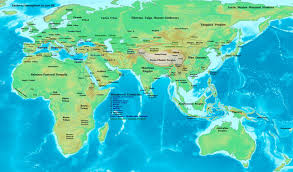
\includegraphics[width=4in]{gecko}
	\caption[Close up of \textit{Hemidactylus} sp.]
	{Close up of \textit{Hemidactylus} sp., which is
		part the genus of the gecko family. It is the
		second most speciose genus in the family.}
	
\end{figure}

\begin{figure}[hb]
	
	\centering
	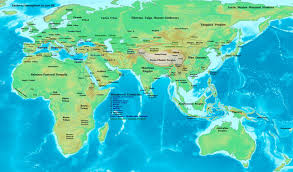
\includegraphics[width=4in]{gecko}
	\caption[Close up of \textit{Hemidactylus} sp.]
	{Close up of \textit{Hemidactylus} sp., which is
		part the genus of the gecko family. It is the
		second most speciose genus in the family.}
	
\end{figure}

\noindent Thank you for reading these instructions carefully. We look forward to receiving your electronic files!

\begin{table}[h!]
	
	\begin{center}
		\begin{tabular}{| l c r |}
			\hline
			1 & 2 & 3 \\
			4 & 5 & 6 \\
			7 & 8 & 9 \\
			\hline
		\end{tabular}
	\end{center}
	\caption{A simple table}
	
\end{table}

\section{Copyright}
All papers submitted for publication by AAAI Press must be accompanied by a valid signed copyright form or, in the case of technical reports, by a valid signed permission to distribute form. There are no exceptions to this requirement. You must send us the original version of this form. However, to meet the deadline, you may fax (1-650-321-4457) or scan and e-mail the form (pubforms15@aaai.org) to AAAI by the submission deadline, and then mail the original via postal mail to the AAAI office. \textbf{If you fail to send in a signed copyright or permission form, your paper will not be published.} You will find PDF versions of the AAAI copyright and permission to distribute forms in the author kit.

\bigskip
\noindent Thank you for reading these instructions carefully. We look forward to receiving your electronic files!

\section{Copyright Copy}
All papers submitted for publication by AAAI Press must be accompanied by a valid signed copyright form or, in the case of technical reports, by a valid signed permission to distribute form. There are no exceptions to this requirement. You must send us the original version of this form. However, to meet the deadline, you may fax (1-650-321-4457) or scan and e-mail the form (pubforms15@aaai.org) to AAAI by the submission deadline, and then mail the original via postal mail to the AAAI office. \textbf{If you fail to send in a signed copyright or permission form, your paper will not be published.} You will find PDF versions of the AAAI copyright and permission to distribute forms in the author kit.

\bigskip
\noindent Thank you for reading these instructions carefully. We look forward to receiving your electronic files!

\end{document}
